%!TEX root = ../main.tex

\begin{figure}
	\centering
	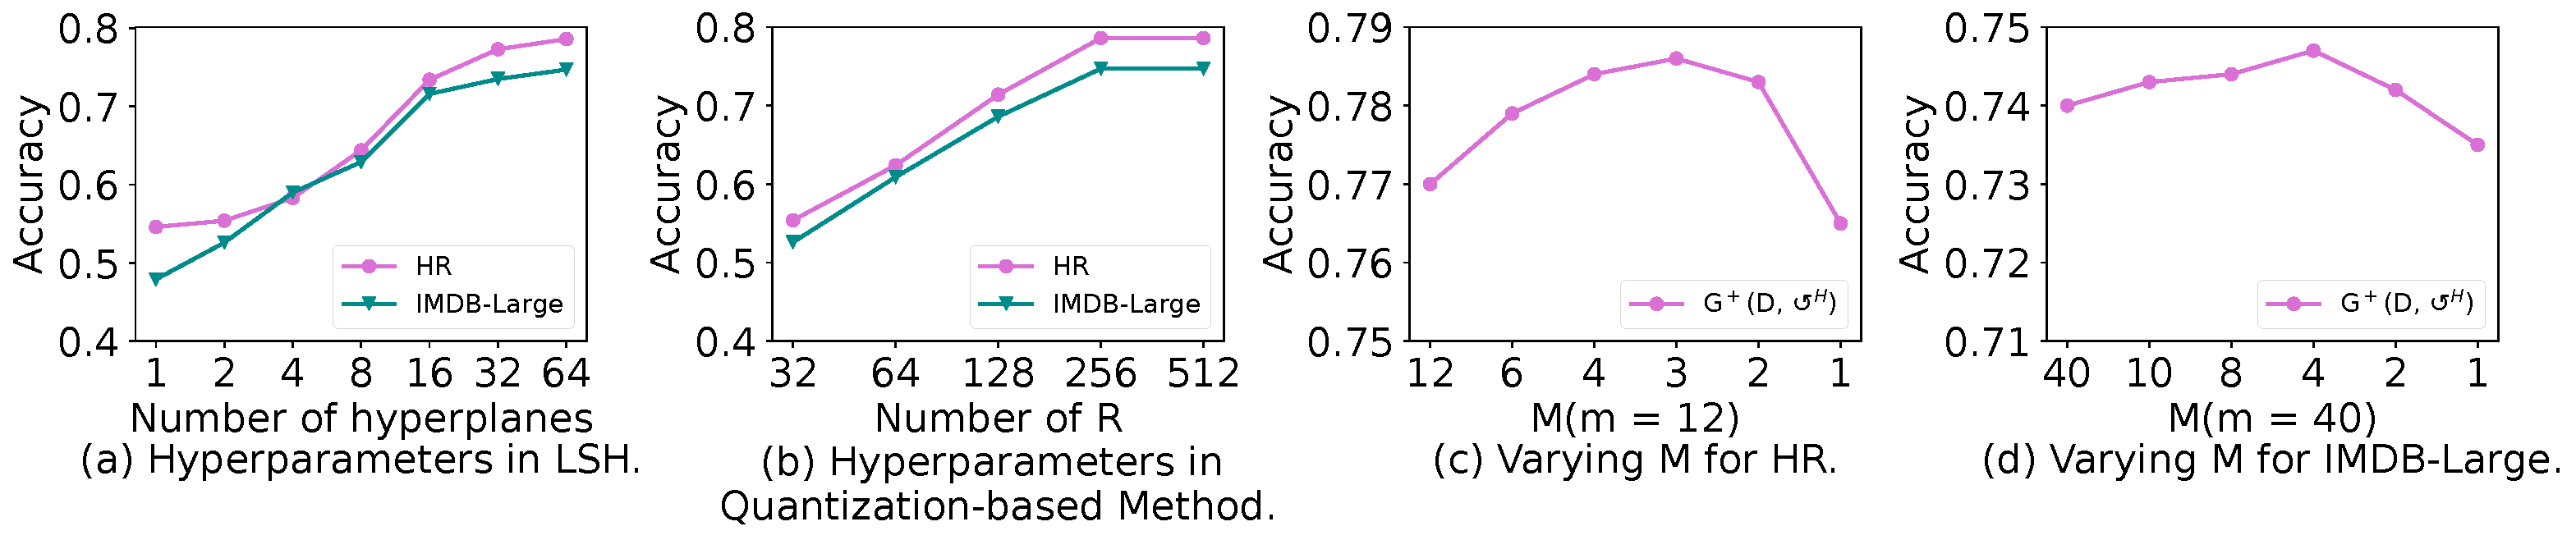
\includegraphics[width=1\textwidth]{figs/M}
	\vspace{-1em}
	\caption{Varying Hyperparameters in LSH and Quantization-based Method.}
	\label{fig:pq-exp}
	\vspace{-1em}
\end{figure}

\subsection{Ablation Studies of \texttt{GoodCore}$^+$}
\noindent{\bf Hyperparamaters for grouping.}
%
We use LSH to efficiently group the entire dataset, and test the impact of  different numbers of hyperplanes, which is a significant parameter in LSH.
 As shown in Figure~\ref{fig:pq-exp} (a), with the number increasing, more groups are generated, and the tuples within each group are closer, so the  accuracy increases at the beginning. Afterwards, the accuracy remains stable because tuples in each cluster are similar enough for  approximating the gradient. Therefore, empirically, using  64 hyperplanes is the most appropriate because more groups will reduce the efficiency.

\noindent{\bf Hyperparamaters in quantization-based method.} In Section~\ref{subsec:pq}, we use quantization-based method to estimate the upper bound $\hat{s}_{ju}$ of $\overline{s}_{ju}$. Recap that \texttt{GoodCore}$^+$ needs the user-specified cluster centers size $R$, which is important for computing the maximum feature distances.
%
 To choose a proper $R$, we adopt a simple yet effective solution that selects different $R$ and obtain different coresets. Then we train over these coresets and evaluate via a validation set to get different results. Specifically, we select $R$ from 32 to 512 for each dataset. Figure~\ref{fig:pq-exp} (b) shows the performance on dataset \hr and \imdbl when varying the cluster centers size $R$.  We can see that as $R$ increases, the accuracy of the dataset also gradually increases, because when $R$ increases, the upper bound $\hat{s}_{ju}$ is closer to $\overline{s}_{ju}$, which can help us to select a good coreset.


We also test the performance of different feature splitting ways (corresponding to different $M$). In Figure~\ref{fig:pq-exp}(c)-(d), initially,  $M=12$ indicates that in each subspace, the length of all sub-vectors is 1. With $M$ decreasing, the accuracy increases first because each sub-vector becomes longer, which contains more information when adding up these $\hat{s}^z_{ju}$, leading to a more precise bound. But if each sub-vector is too long, which means that each vector is quantized to a very short code, the accuracy decreases because in this situation, the quantization-based method is not informative enough to give accurate  distance estimation. Empirically, when $M$ is around 3, it is always a good choice.

\noindent{\bf Varying the entropy threshold.} 
\begin{figure}[t]   
	\centering
	\begin{minipage}[t]{0.3\textwidth}
		\centering
		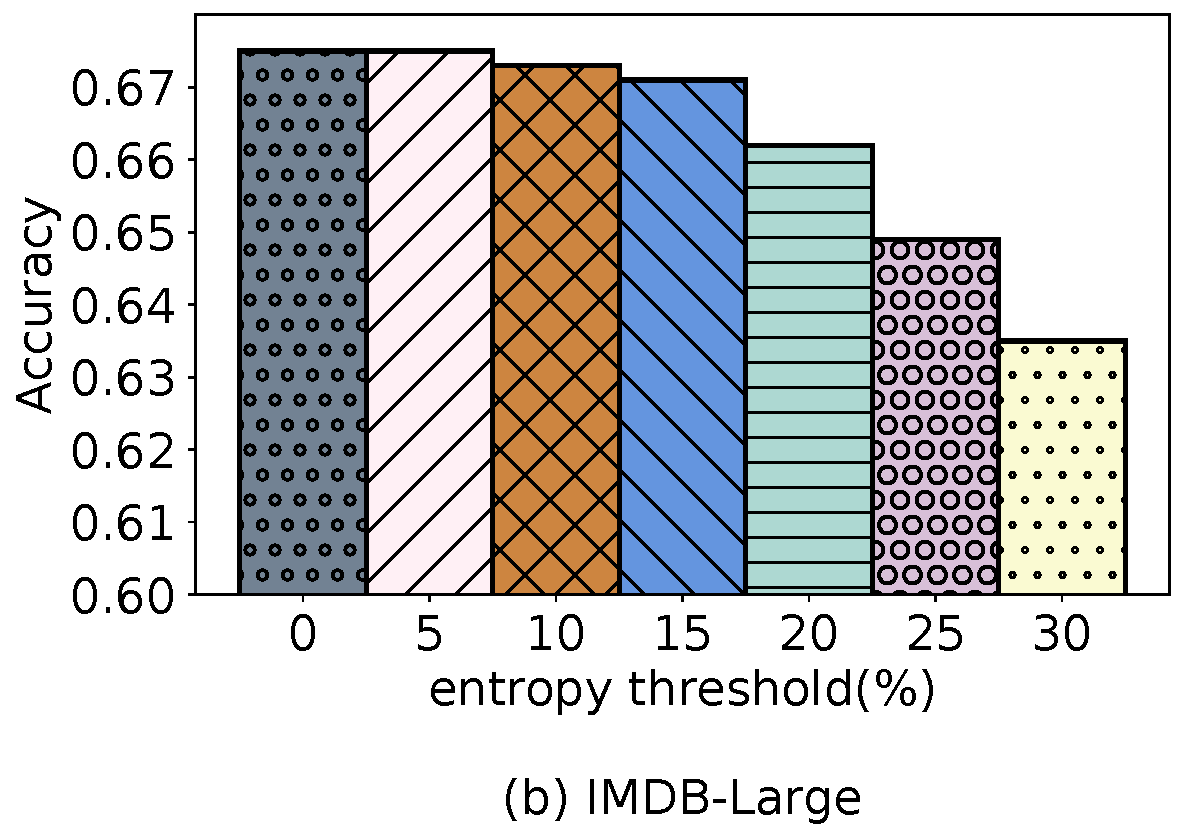
\includegraphics[width=\columnwidth]{figs/entropy_acc}
		\vspace{-1.5em}
		\caption{Effectiveness of \ours$^+$ for different Threshold.}
		\label{fig:entropy_acc}
	\end{minipage}
	\begin{minipage}[t]{0.3\textwidth}
		\centering
		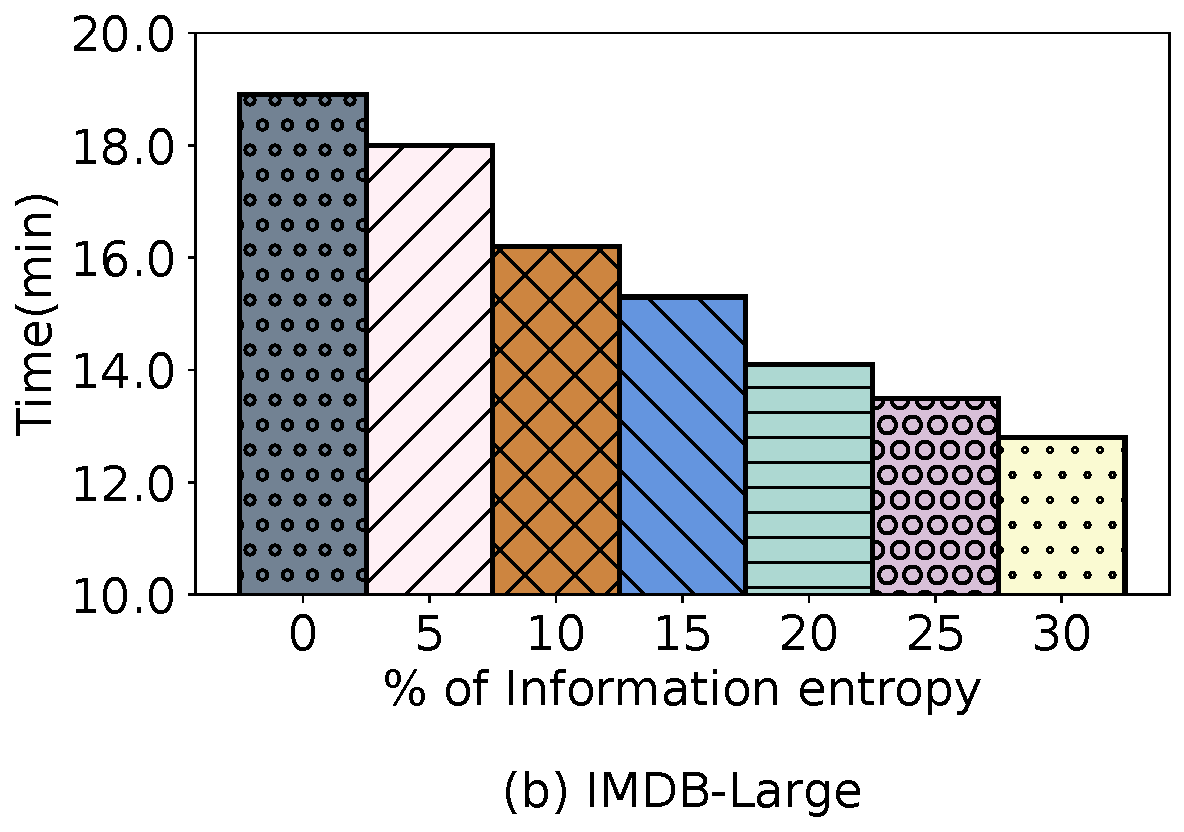
\includegraphics[width=\columnwidth]{figs/entropy_time}
		\vspace{-1.5em}
		\caption{Efficiency of \ours$^+$ for different Threshold.}
		\label{fig:entropy_time}
	\end{minipage}
	\vspace*{-1em}   
\end{figure}
%
In this part, we start to use the entropy to further eliminate the number of possible world by imputing the missing cells with low entropy in advance, as discussed in Section~\ref{subsec:clustering}. 
%
Specifically, we test the impact of different entropy thresholds. As shown in Figure~\ref{fig:entropy_acc} and Figure~\ref{fig:entropy_time}, when the threshold is less than  20\% (\ie we directly impute the cell if its corresponding entropy is no larger than 20\% $\log n_x$), the accuracy almost remains unchanged, while the efficiency is improved by up to 20\%. However, when the threshold exceeds 20\%, the accuracy begins to decrease because in this situation, directly imputing a value is not accurate enough. In short, setting an appropriate threshold (\eg 20\%) is helpful to improve the efficiency without sacrificing the accuracy. 

% rate of decrease accelerates. This is because when the threshold is low, all the candidate words filled in for the missing values have a high probability(\ie 90\%) and the threshold increases, the maximum probability gradually decreases, making the selection of candidate words for missing values more challenging. For example, on dataset \imdbl, when threshold is 15\%, the accuracy of \ours$^+$ is 71\%, which is only 0.4\% lower than when no processing is done at all.

%Furthermore, we report the time change to reflect the efficiency of \ours$^+$ for different thresholds of information entropy. In Figure~\ref{fig:entropy_time}, we can see that the algorithm spends less and less time as the threshold increases because of the reduction in the number of incomplete tuples. On dataset \imdbl, when threshold is 30\%, the runtime of \ours$^+$ has decreased by over 30\%. And the runtime of \ours$^+$ decreased by approximately 3 minutes when threshold is 15\%.
%
%In summary, we can use a appropriate threshold of information entropy to preemptively fill in some missing values, which can effectively reduce the runtime of \ours$^+$ while ensuring accuracy. 
